
% \usepackage{graphicx}
% \usepackage{subfigure}
% \usepackage{amsmath}
% %\usepackage{amsxtra}
% %\usepackage{amstext}
% \usepackage{amssymb}
% %\usepackage{amscd}
% %\usepackage{amsthm}

% %\usepackage{authblk}

% %\newtheorem{remark}{Remark}
% %\newtheorem{definition}{Definition}
% %\newtheorem{proposition}{Proposition}
% %\newtheorem{corollary}{Corollary}

% \newcommand{\tr}[1]{\mbox{tr}(#1)}
% \newcommand{\vol}[0]{\mbox{vol}}

% \newcommand{\prob}[1]{\mathbb{P}\left[#1\right]}
% \newcommand{\expect}[1]{\mathbb{E}\left[#1\right]}
% \newcommand{\expb}[1]{\exp\left(#1\right)}
% \newcommand{\indicator}[1]{\mathbb{I}_{#1}}
% \newcommand{\pd}[1]{\frac{\partial}{\partial #1}}
% \newcommand{\pdd}[1]{\frac{\partial^2}{\partial #1^2}}

% \newcommand{\image}{\mathop{\mathrm{im}}
% \newcommand{\preimage}{\mathop{\mathrm{pre}}
% \newcommand{\Hom}{\mathop{\mathrm{Hom}}
% \newcommand{\Ext}{\mathop{\mathrm{Ext}}

% \newcommand{\VR}{\mathop{\mathrm{VR}}
% \newcommand{\LW}{\mathop{\mathrm{LW}}


%\newcommand{\address}[1]{\subsubsection*{\it#1}}



\title{javaPlex: A research software package for persistent (co)homology}
\titlerunning{javaPlex}
\author{Henry Adams\inst{1}
\and Andrew Tausz\inst{2}
\and Mikael Vejdemo-Johansson\inst{3,4}}

\institute{Institute of Mathematics and its
  Applications, USA \and Stanford University, USA \and KTH Royal Institute of Technology, Sweden, \\
  \texttt{mvj@kth.se} \and
  Institut Jozef Stefan, Slovenia}

\date{\today}


\maketitle

\begin{abstract}
The computation of persistent homology has proven a fundamental component of the nascent field of topological data analysis and computational topology. We describe a new software package for topological computation, with design focus on needs of the research community. This tool, replacing previous jPlex and Plex, enables researchers to access state of the art algorithms for persistent homology, cohomology, hom complexes, filtered simplicial complexes, filtered cell complexes, witness complex constructions, and many more essential components of computational topology.

We describe, herewithin, the design goals we have chosen, as well as the resulting software package, and some of its more novel capabilities.

%In this document, we describe the design and goals of the javaPlex
%software package. Its main purpose is to support research in the area
%of topological data analysis; the two main capabilities being the
%construction of filtered chain complexes of vector spaces, and the
%computation of their persistent homology.
\keywords{persistent homology, topological data analysis,
  computational topology}
\end{abstract}

\section{Motivation and Design Goals}

The main reason for the existence of javaPlex is to provide researchers in the area of topological data analysis a unified software library to support their investigations. With this in mind, the design goals for it are as follows:

\begin{itemize}
\item {\bf Support for new directions for research: } The main goal of the javaPlex package is to provide an extensible base to support new avenues for research in computational homology and data analysis. While its predecesor jPlex was very well suited towards computing simplicial homology, its design made extension difficult.
\item {\bf Interoperability: } Since javaPlex is a java package, it is
  accessible from anything that runs in the Java runtime environment:
  in a Java or Scala application, or called from Matlab or Mathematica, or as a
  library loaded into beanshell, jython for a scripting interface.
\item {\bf Adherence to generally accepted software engineering practices: } As a means to realizing the first goal, the javaPlex software package was designed and implemented with software engineering best-practices. Emphasis was placed on maintainability, modularity, and reusability of the different parts of the code.
\end{itemize}

We refer the reader to \cite{Carlsson_09} for a very readable introduction to the field of topological data analysis as well as the computational tasks involved.

\section{Previous Work}

The javaPlex package is the fourth version in the Plex family. These programs have been developed over the past decade by members of the computational topology research group at Stanford University. Each successive version incorporated the results of new advances in the relatively quickly developing fields of computational topology and topological data analysis.

Like javaPlex, its predecessor jPlex was also written in the Java language. However, it differed in that the main goal of jPlex was the computation of \emph{simplicial} homology. Recent research topics in topological data analysis have required practitioners to move beyond conventional simplicial homology to more general scenarios.

\section{Persistent homology and topological data analysis}
\label{sec:pers-homol-topol}

The javaPlex library is focused on computing persistent homology and
enabling research and use of topological data analysis methods. At the
core of these tasks is the ability to compute the homology indicated
by a point cloud. To this end, \cite{ELZ_02} introduced persistent homology, refined by
\cite{Carlsson_04}. Using one of a whole family of methods, the point
cloud induces a filtered simplicial complex, where the filtration
encodes distance data as increasing ``closeness'' data for the data
points in the point cloud. From a simplicial complex, we can generate
a \emph{chain complex}: a vector space with vectors representing the
geometry and with an operator $\partial$ capturing what it means to be on the
boundary of a cell. The homology is defined as
$\ker\partial/\mathop{\mathrm{im}}\partial$, and can be considered to represent
\emph{essential cycles} or \emph{bubbles} in arbitrary high dimensions
as witnessed in the data itself.

Persistence captures the notion of computing this homology for a range
of parameter values, connecting the local results to extract a
\emph{barcode} that represents each such essential feature as a
discrete component coupled with a spread of parameter values at which
the feature exists in the dataset. For more details, we refer an
interested reader to \cite{Carlsson_09}.

\section{Filtered Complex Generation}

As mentioned in the abstract, the primary function of javaPlex is the construction of filtered chain complexes of vector spaces associated to actual point cloud datasets. The motivation for such constructions is that they provide a persistent model of the dataset in question across all scales. javaPlex currently supports the construction of two main types of filtered simplicial complexes: the Vietoris-Rips and lazy-witness constructions. To begin, suppose that we have a finite metric space $(\mathcal{X}, d)$. In practice, it is possible that $\mathcal{X}$ is a set of points in Euclidean space, although this is not necessary.

\subsection{The Vietoris-Rips Construction}
We define the filtered complex $\mathop{\mathrm{VR}} (\mathcal{X}, r)$ as follows. Suppose that the points of $\mathcal{X}$ are $\{x_1, ... x_N\}$, where $N = |\mathcal{X}|$. The Vietoris-Rips complex is constructed as follows:

\begin{itemize}
\item {\bf Add points:} For all points $x \in \mathcal{X}$, $x \in \mathop{\mathrm{VR}}_0(\mathcal{X}, 0)$.
\item {\bf Add 1-skeleton:} The 1-simplex $[x_i, x_j]$ is in $\mathop{\mathrm{VR}}_1(\mathcal{X}, r)$ iff $d(x_i, x_j) \leq r$.
\item {\bf Expansion:} We define $\mathop{\mathrm{VR}} (\mathcal{X}, r)$ to be the maximal simplicial complex with 1-skeleton $\mathop{\mathrm{VR}}_1(\mathcal{X}, r)$. That is, a simplex $[x_0, .. x_k]$ is in $\mathop{\mathrm{VR}} (\mathcal{X}, r)$ if and only if all of its edges are in $\mathop{\mathrm{VR}}_1(\mathcal{X}, r)$.
\end{itemize}

An extensive discussion on algorithms for computing the Vietoris-Rips complex can be found in \cite{Zomorodian}. The javaPlex implementation is based on the results of this paper.

\subsection{The Lazy-Witness Construction}
The fundamental idea behind the lazy-witness construction is that a relatively small subset of a point cloud can accurately describe the shape of the dataset. This construction has the advantage of being more resistant to noise than the Vietoris-Rips construction. An extensive discussion about it can be found in \cite{Witness}. 

The lazy-witness construction starts with a selection of landmark points, $\mathcal{L} \subset \mathcal{X}$ with $|\mathcal{L}| = L$. One possibility is to simply choose a random subset of $\mathcal{X}$. Another possibility is to perform a sequential max-min selection: An initial point $l_0$ is selected, and then we inductively select the point $l_k$ which maximizes the minimum distance to all previously generated points. This max-min construction tends to produce more evenly spaced points than the random selection. Again we refer the reader to \cite{Witness} for a more detailed discussion, as well as empirical results supporting these claims.

This construction is parameterized by a value $\nu$, which most commonly takes the values 0, 1, or 2. We also define the distance matrix $D$ to contain the pairwise distances between the points in $\mathcal{X}$. 

\begin{itemize}
\item {\bf Define $m_i$:} If $\nu = 0$, let $m_i = 0$, otherwise, define $m_i$ to be the $\nu$-th smallest entry in the $i$-th column of $D$.
\item {\bf Add points:} For all points $l \in \mathcal{L}$, $l \in \mathop{\mathrm{LW}}_0(\mathcal{X}, 0, \nu)$.
\item {\bf Add 1-skeleton:} The 1-simplex $[l_i, l_j]$ is in $\mathop{\mathrm{LW}}_1(\mathcal{X}, r, \nu)$ iff there exists an $x \in \mathcal{X}$ such that $\max(d(l_i, x), d(l_j, x)) \leq r + m_i$.
\item {\bf Expansion:} We define $\mathop{\mathrm{LW}} (\mathcal{X}, r, \nu)$ to be the maximal simplicial complex with 1-skeleton $\mathop{\mathrm{LW}}_1(\mathcal{X}, r, \nu)$. 
\end{itemize}

\section{Homology Computation}

At the core of the javaPlex library is the set of algorithms that actually compute the homology of a filtered chain complex. Key references to background material regarding these algorithms can be found in \cite{Carlsson_04,Dualities}. Although we do not describe them in detail here, we note that the algorithms for computing persistent absolute/relative (co)homology can be formulated as matrix decomposition problems. The fundamental reason for this is the equivalence of the category of persistent vector spaces of finite type, and the category of finitely generated graded modules over $\mathbb{F}[t]$. This correspondence is described in \cite{Carlsson_04}. 

The homology algorithms are built in a way that is optimized for chain complexes implemented as \emph{streams}. By this we mean that a filtered chain complex is represented by a sequence of basis elements that are produced in increasing order of their filtration indices. Enforcing the constraint that all complexes must be implemented this way allows javaPlex to perform the matrix decomposition operations in an efficient online fashion.

\section{Applications}

Although in principle javaPlex can compute the persistent homology of arbitrary chain complexes of vector spaces, almost always these complexes arise from some sort of topological construction. Below we outline these different situations.

\subsection{Simplicial Homology}
\label{sec:simplicial-homology}

Computing simplicial homology of a filtered sequence of complexes is
performed by generating a \texttt{SimplexStream} and running it
through the persistent homology algorithm. A sample invocation would look
like follows:

\begin{verbatim}
 ExplicitSimplexStream stream = new ExplicitSimplexStream();
 // add vertices with stream.addVertex; simplices with
 // stream.addElement
 stream.finalizeStream();
 AbstractPersistenceAlgorithm<Simplex> pA = 
   Plex4.getDefaultSimplicialAlgorithm(d + 1);
 BarcodeCollection<Double> intervals = pA.computeIntervals(stream);
\end{verbatim}

\subsection{Simplicial Cohomology}
\label{sec:simpl-cohom-1}

As described in \cite{Dualities}, persistent cohomology can be
computed by consuming simplices in the opposite order, computing
coboundaries instead of boundaries, and reversing the order of
simplices when picking out leading terms. This is supported in
javaPlex through the \texttt{DualStream} class that transforms an
existing simplex stream to a reversed version, together with the Java
utility method
\texttt{java.util.Collections.reverseOrder} which can reverse the
simplex order declaration instantiating the homology algorithm:

\begin{verbatim}
 AbstractPersistenceAlgorithm<Simplex> pA = 
   new IntAbsoluteHomology(ModularIntField.getInstance(prime), 
          Collections.reverseOrder(SimplexComparator.getInstance()), 
          0, d+1);
 BarcodeCollection<Double> intervals = pA.computeIntervals(stream);
\end{verbatim}

\subsection{Novel operations and types}
\label{sec:novel-oper-types}

javaPlex also supports arbitrary cell complexes, where the gluing maps
are given explicitly rather than generating them implicitly from the
simplices. In addition to this, there is also support for computing
with \textbf{tensor products} and \textbf{Hom complexes} of chain
complexes of any type in the system. The particular case of dualizing
a chain complex to get cochains is handled by \texttt{DualStream},
while the general homomorphism complexes are handled by
\texttt{HomStream} instead.

In a recent preprint \cite{hom}, the hom-complex was used to compute a parameterization for the space of homotopy classes of chain maps between simplicial complexes.


\section{Examples}

\subsection{Simplicial Homology}

In Figure \ref{lwtorus}, one can see an example of a filtered simplicial complex generated from points on a torus. As one moves from left to right, the filtration parameter $r$ is increased, yielding a more connected complex. In Figure \ref{lwtorusbarcodes} we show the persistence barcodes for the same shape. Note that the significant intervals correspond to homological features that last for a long time in the filtration.

\begin{figure}
\centering
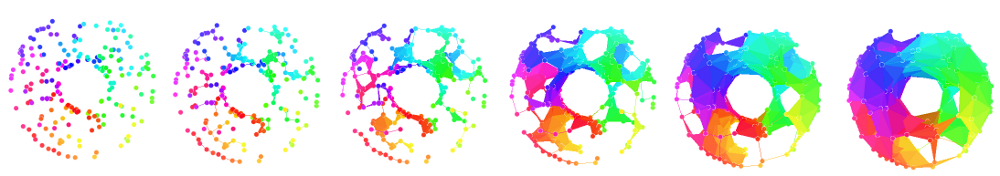
\includegraphics[width=0.9\textwidth]{Adams_Henry/images/tori_small.png}
\caption{Example of a lazy-witness complex generated from randomly sampled points on a torus.} \label{lwtorus}
\end{figure}

\begin{figure}
\centering
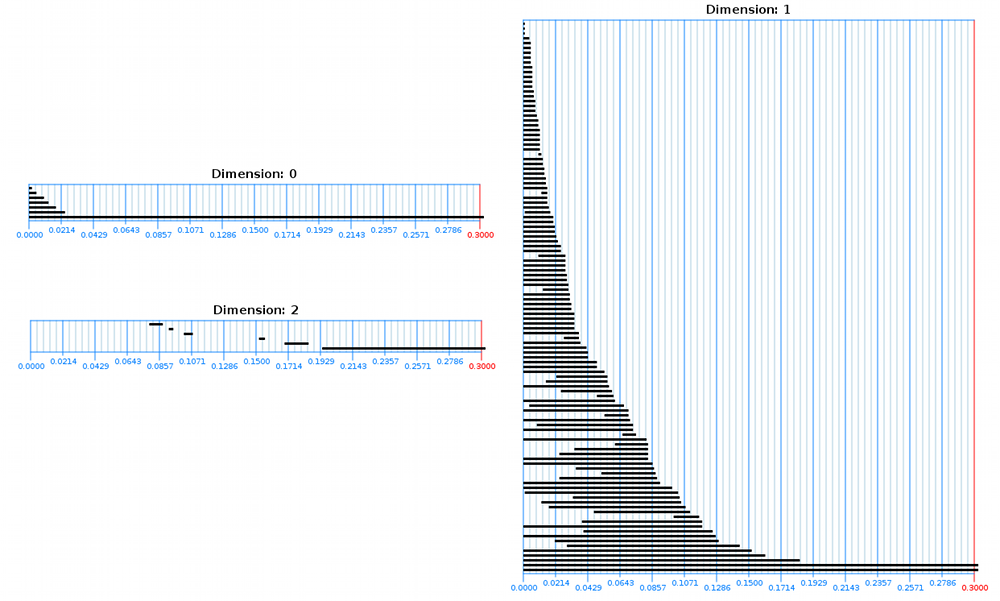
\includegraphics[width=0.9\textwidth]{Adams_Henry/images/barcodes_small.png}
\caption{Persistence barcodes for a lazy-witness filtration of random points on a torus. The parameters used were: $N = 1000$, $L = 300$, $r_{\max} = 0.3$. The inner and outer radii of the torus were 0.5 and 1, respectively. The max-min selection procedure was used to create the landmark set. Note that long intervals correspond to significant homological features, and short ones are most likely the result of noise. We can see that the number of significant intervals in each dimension equals the expected Betti number.} \label{lwtorusbarcodes}
\end{figure}

\subsection{Matlab Scripting Example - Cellular Homology}

In this section we show a brief Matlab session in which the cellular homology is computed for a Klein bottle over different coefficient fields. Essentially, this code example constructs a cellular Klein bottle, initializes persistence algorithm objects over the fields $\mathbb{Z}/2\mathbb{Z}$, $\mathbb{Z}/3\mathbb{Z}$, and $\mathbb{Q}$, and computes the persistence intervals.

\begin{verbatim}
% get the cellular Klein bottle
stream = examples.CellStreamExamples.getCellularKleinBottle();

% get cellular homology algorithm over Z/2Z
Z2_persistence = api.Plex4.getModularCellularAlgorithm(3, 2);
% get cellular homology algorithm over Z/3Z
Z3_persistence = api.Plex4.getModularCellularAlgorithm(3, 3);
% get cellular homology algorithm over Q
Q_persistence = api.Plex4.getRationalCellularAlgorithm(3);

% compute over Z/2Z - should give (1, 2, 1)
Z2_intervals = Z2_persistence.computeIntervals(stream)

% compute over Z/3Z - should give (1, 1, 0)
Z3_intervals = Z3_persistence.computeIntervals(stream)

% compute over Q - should give (1, 1, 0)
Q_intervals = Q_persistence.computeIntervals(stream)
\end{verbatim}
The output of this example is:
\begin{verbatim}
Z2_intervals =
Dimension: 2 [0, infinity)
Dimension: 1 [0, infinity), [0, infinity)
Dimension: 0 [0, infinity)
  
Z3_intervals =
Dimension: 1 [0, infinity)
Dimension: 0 [0, infinity)
 
Q_intervals =
Dimension: 1 [0, infinity)
Dimension: 0 [0, infinity)
\end{verbatim}
This is exactly what we expect, due to the presence of 2-torsion in the Klein bottle.

\subsection{Hom Complex Examples}

As mentioned earlier, the hom complex is another homological construction that is useful in algebraic topology. A key result is that the 0-dimensional homology classes of $\mathop{\mathrm{Hom}}(A,B)_*$ correspond exactly with homotopy classes of chain maps between $A$ and $B$. Thus, by computing homology (with field coefficients in our case), we can obtain an explicit parameterization of the affine space of homotopy classes of chain maps for simplicial complexes. Additionally, a practitioner can also optimize over this space to select a particular map that optimizes some sort of geometric objective.

In Figures \ref{hom_circle} and \ref{hom_trefoil} we show examples of the computation of homotopy representatives of chain maps between two simplicial complexes. The specific maps were computed by minimizing the maximum $\ell_1$ norm of the images and adjoint images. The maps are represented by composing the color of the domain with the computed map. In the first example we can see that the larger circle is essentially partitioned into different segments of constant color. The second example shows the mapping of a trefoil knot to a square.

\begin{figure}
\centering
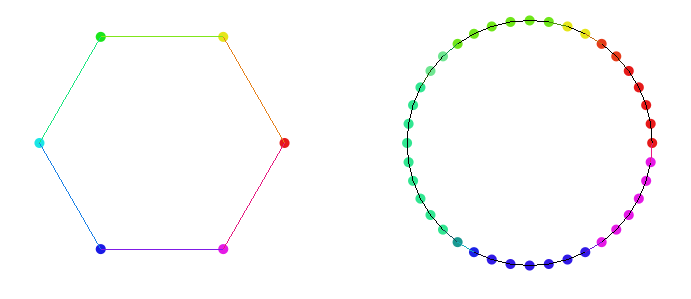
\includegraphics[width=0.5\textwidth]{Adams_Henry/images/hom_circle.png}
\caption{Example of a homotopy representative from the class of chain maps that induce isomorphisms on both 0 and 1 dimensional homology.} \label{hom_circle}
\end{figure}

\begin{figure}
\centering
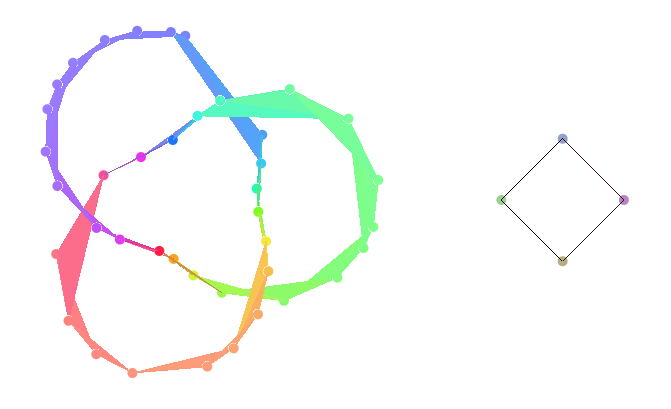
\includegraphics[width=0.5\textwidth]{Adams_Henry/images/hom_trefoil.png}
\caption{Example of a chain map on a lazy-witness filtration of a trefoil knot.} \label{hom_trefoil}
\end{figure}

\begin{thebibliography}{4}
\bibitem[Car09]{Carlsson_09}
Gunnar Carlsson, \emph{{Topology and data}}, Bulletin of the American
  Mathematical Society \textbf{46} (2009), no.~2, 255--308.

\bibitem[dSC04]{Witness}
Vin de~Silva and Gunnar Carlsson, \emph{{Topological estimation using witness
  complexes}}, Eurographics Symposium on Point-Based Graphics (M.~Alexa and
  S.~Rusinkiewicz, eds.), The Eurographics Association, 2004.

\bibitem[dSMVJ10]{Dualities}
Vin de~Silva, Dmitriy Morozov, and Mikael Vejdemo-Johansson, \emph{{Dualities
  in persistent (co)homology}}, Unpublished manuscript, 2010.

\bibitem[ELZ02]{ELZ_02}
Herbert Edelsbrunner, David Letscher, and Afra Zomorodian, \emph{Topological
  persistence and simplification}, Discrete Comput. Geom. \textbf{28} (2002),
  no.~4, 511--533, Discrete and computational geometry and graph drawing
  (Columbia, SC, 2001). MR 1949898 (2003m:52019)

\bibitem[TC11]{hom}
Andrew Tausz and Gunnar Carlsson, \emph{{Homological Coordinatization}},
  Preprint, 2011.

\bibitem[ZC05]{Carlsson_04}
Afra Zomorodian and Gunnar Carlsson, \emph{Computing persistent homology},
  Discrete Comput. Geom \textbf{33} (2005), 249--274.

\bibitem[Zom10]{Zomorodian}
A.~Zomorodian, \emph{Fast construction of the {V}ietoris-{R}ips complex},
  Computers \& Graphics \textbf{34} (2010), no.~3, 263 -- 271.

\end{thebibliography}